\section{SiteLang Specification}
The following figures show various and distinct flow, structure and behaviour of the web information system from KAFFEESATT web application.
Specifications: On every page there is the navigation bar. Furthermore it is possible to login or logout on every page as well. If user is not log in and want to use a log in feature he will be directed to the login input form.
\begin{figure}[ht]
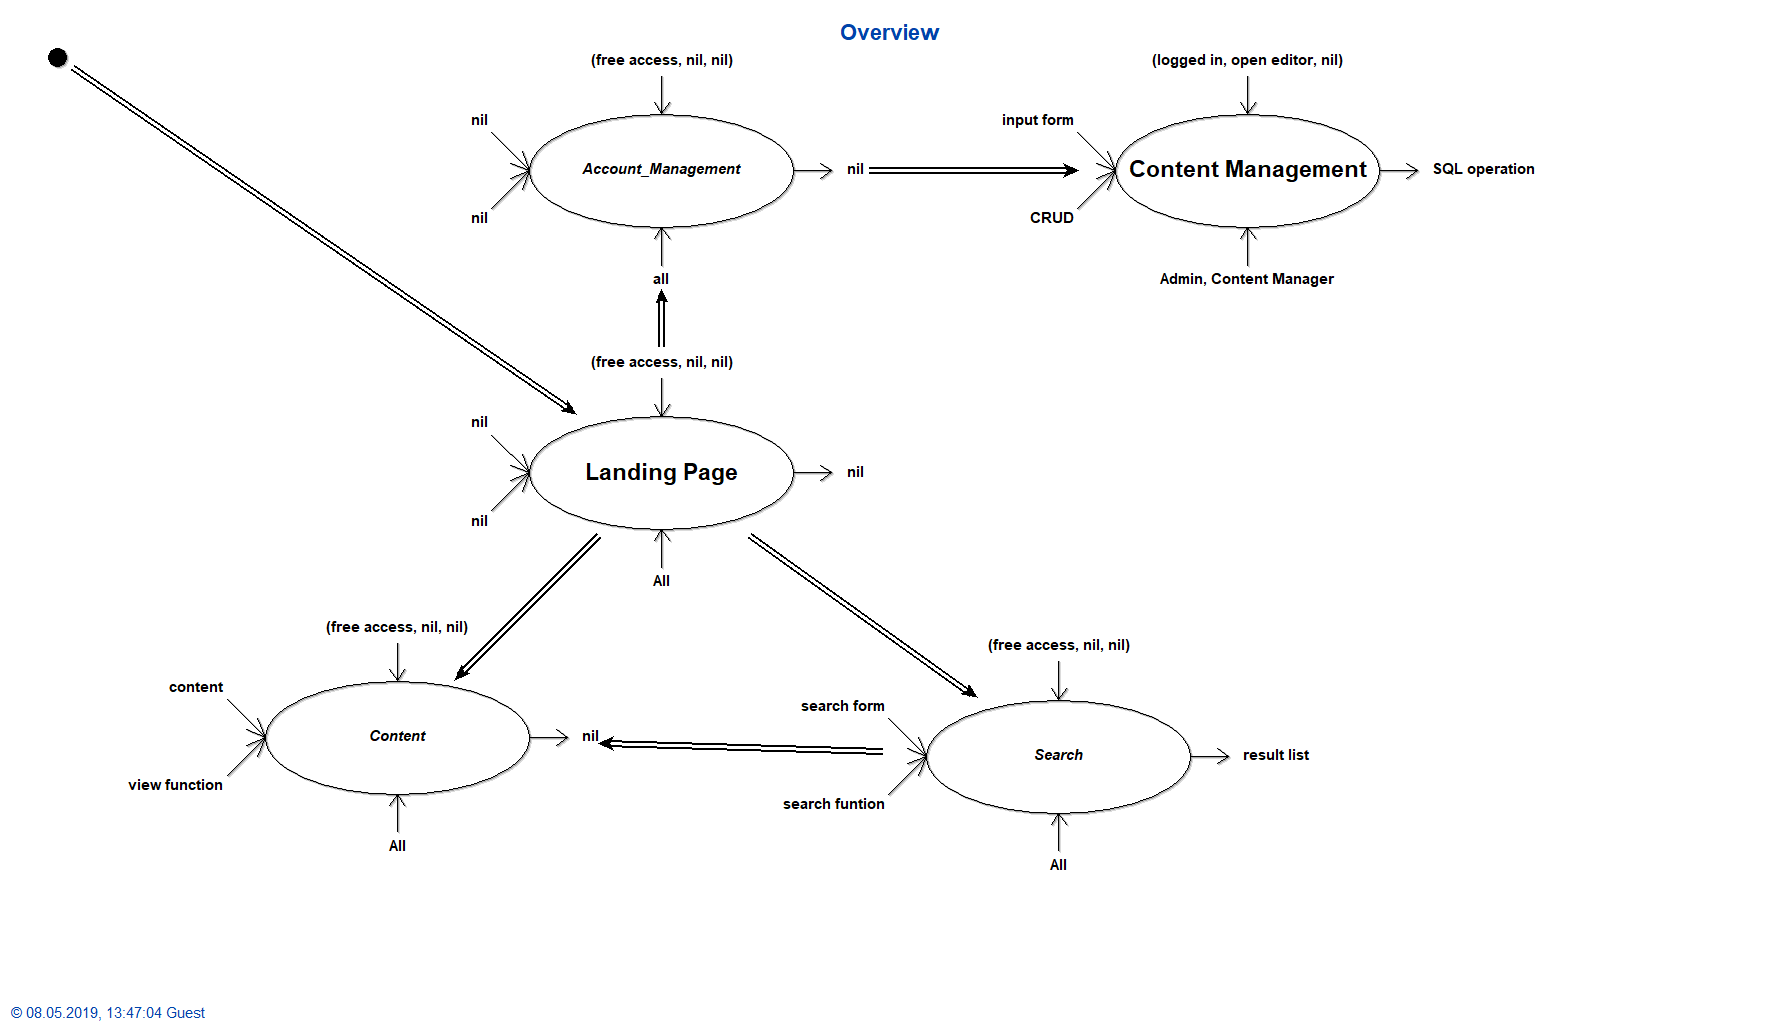
\includegraphics[
    width=\textwidth,
    height=\textheight,
    keepaspectratio
]{Content/SiteLang/Overview.png}
\caption{Overview of KAFFEESATT}
\end{figure}

\begin{figure}[ht]
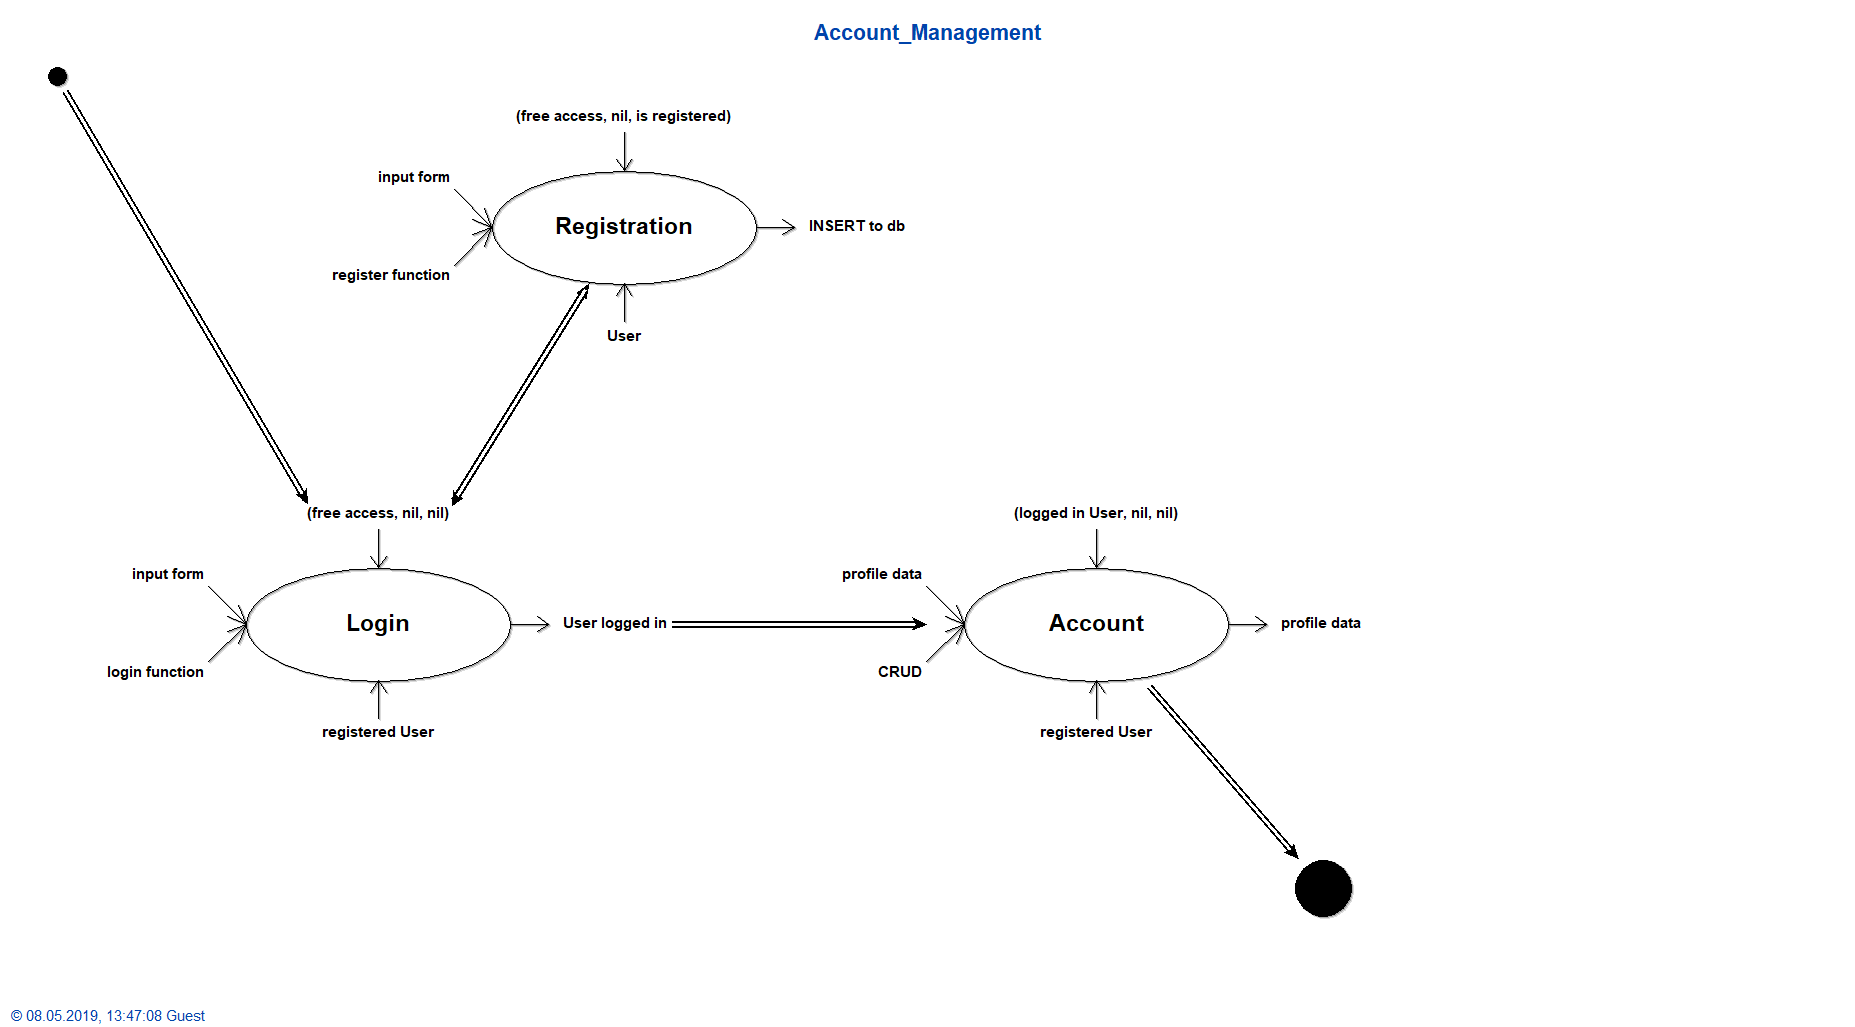
\includegraphics[
    width=\textwidth,
    height=\textheight,
    keepaspectratio
]{Content/SiteLang/Account_Management.png}
\caption{Account Management of KAFFEESATT}
\end{figure}

\begin{figure}[ht]
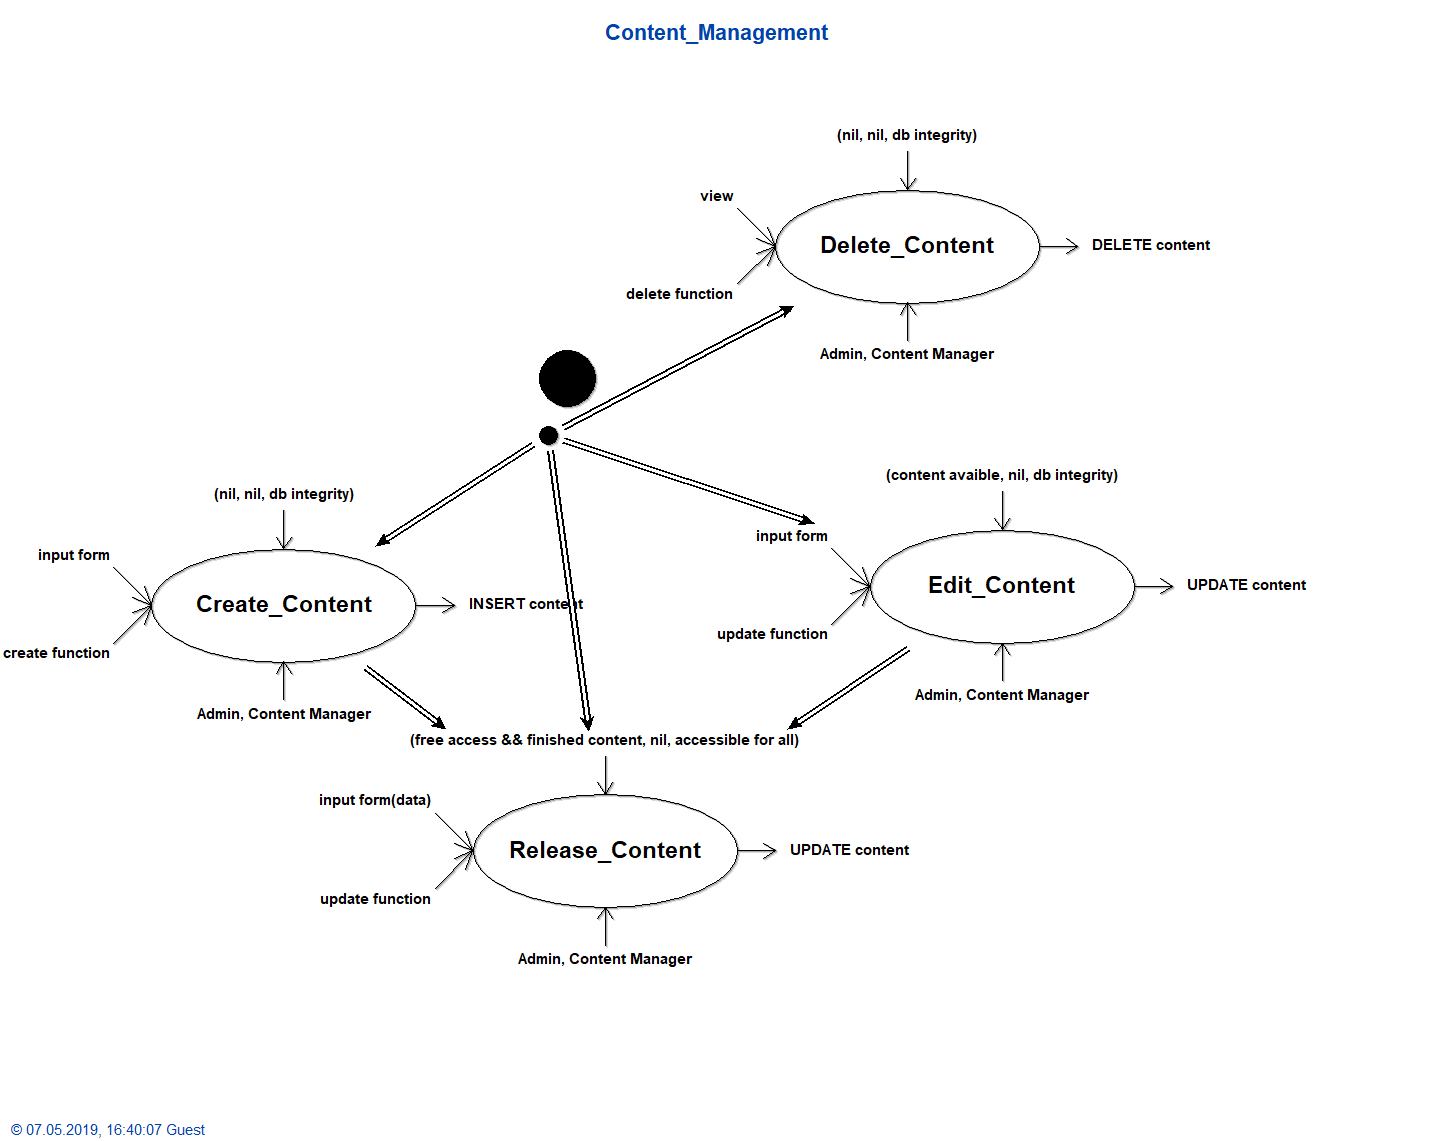
\includegraphics[
    width=\textwidth,
    height=\textheight,
    keepaspectratio
]{Content/SiteLang/Content_Management.png}
\caption{Content Management of KAFFEESATT}
\end{figure}

\begin{figure}[ht]
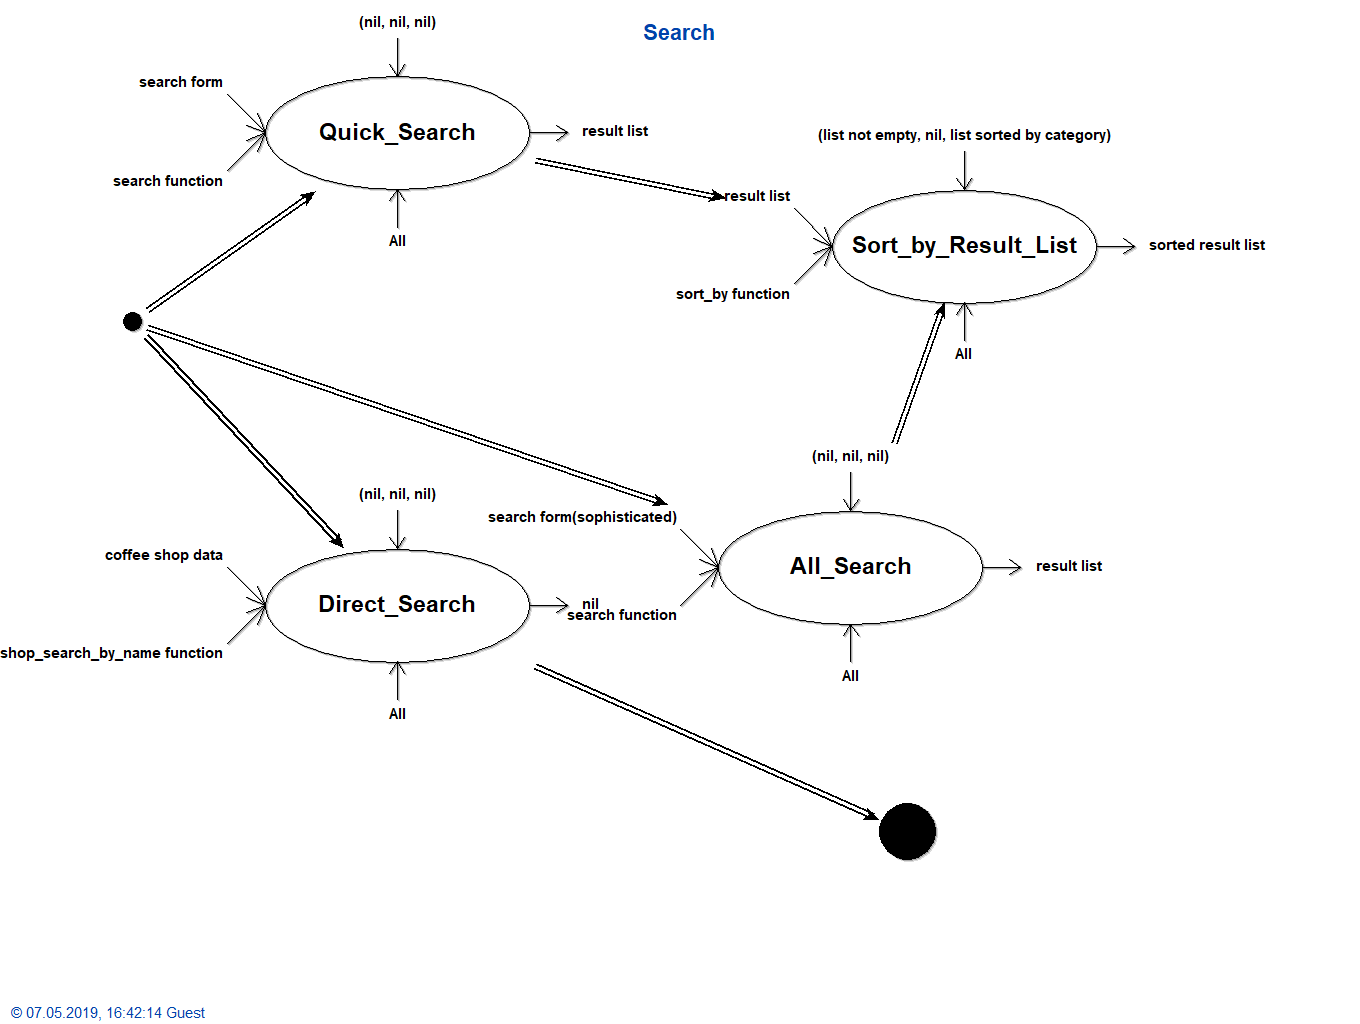
\includegraphics[
    width=\textwidth,
    height=\textheight,
    keepaspectratio
]{Content/SiteLang/Search.png}
\caption{Search of KAFFEESATT}
\end{figure}

\begin{figure}[ht]
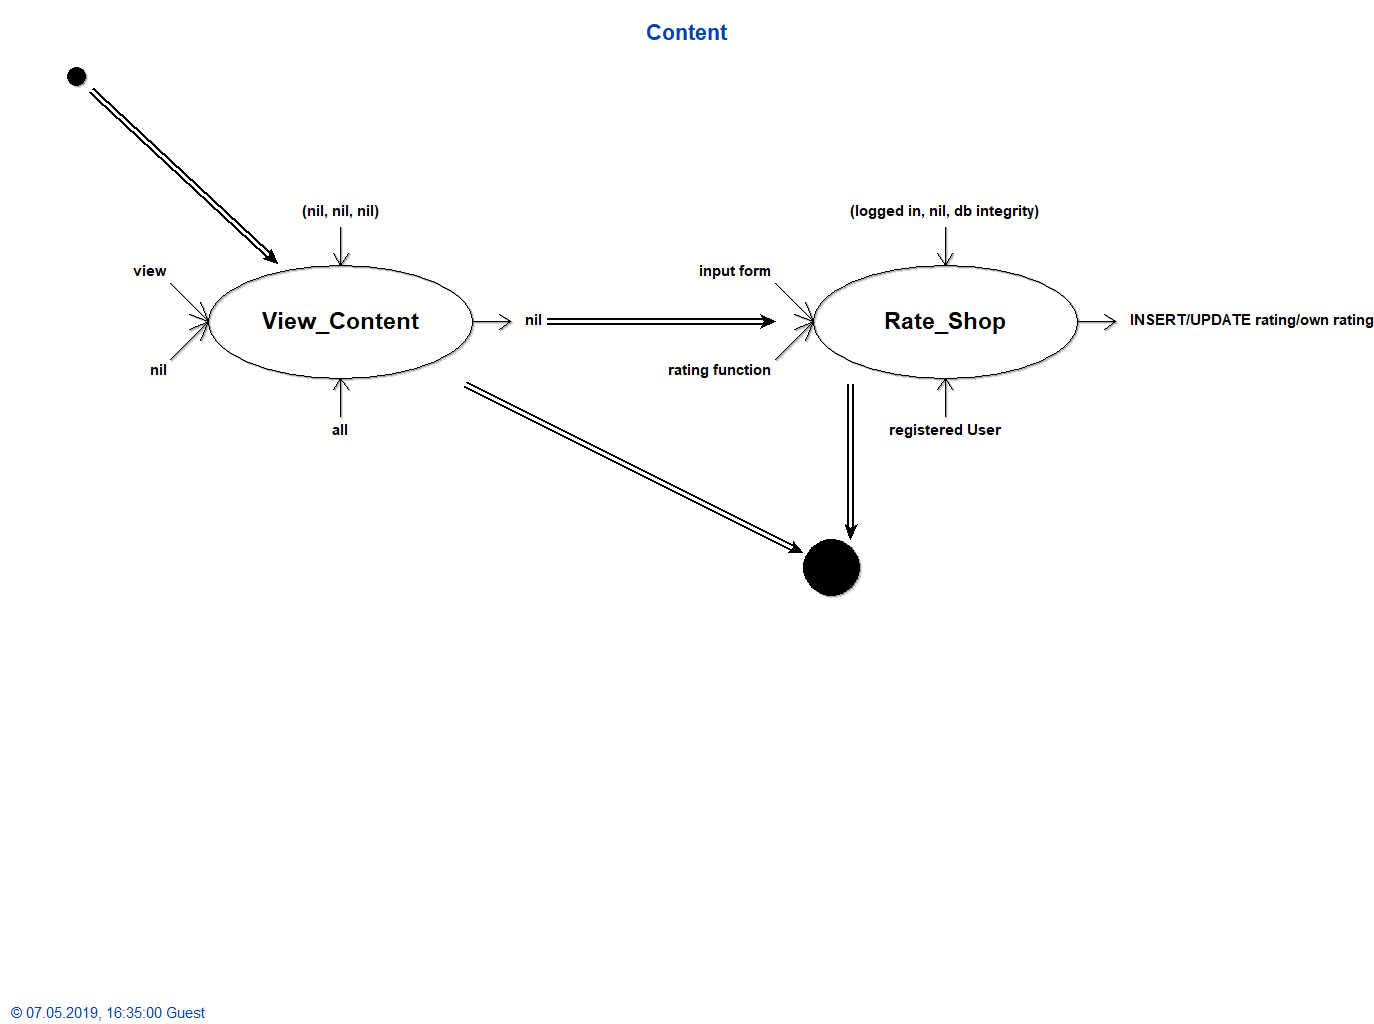
\includegraphics[
    width=\textwidth,
    height=\textheight,
    keepaspectratio
]{Content/SiteLang/Content.png}
\caption{Content KAFFEESATT}
\end{figure}
\clearpage



\subsection{SiteLang Functionality by Scene}
\paragraph{Defintions}

\subparagraph{SETs}
\begin{itemize}
\item Content are the following entities C := \{Shop\} with their following attributes.
\item Article are the following entities A := \{Blend, Beans, Coffee\_Drink, Equipment\}.
\item User    are the following entity   U := \{User and their specialization\}.
\end{itemize}


\subparagraph{FUNCTIONs}
\begin{itemize}
\item $filter:: (C ~\times~ filterContent) \rightarrow Boolean: x \mapsto \textrm{if Content satisfied filter flags: return true; else false;}$
\item $filter:: (A ~\times~ filterArticle) \rightarrow Boolean: x \mapsto \textrm{if Article satisfied filter flags: return true; else false;}$
\item  $filterContent:: C \rightarrow Value: \{C.Attributes\} = $\{poi, workstation, equipment, wlan, outdoor, fair\_trade, child\_friendly, disabled\_friendly, latte\_art, pet\_friendly, food, franchise, price\_class \}
\item  $filterArticle:: A \rightarrow Value: \{A.Attributes\} = $\{category, sub\_category\} 
\item $reduced(filterContent):: \{quickserch(X) | X  \in C.Attributes\} = $\{POI, Workstation, Rösterei \}
\item $id: (C \cup A) -> id: x ->  \textrm{give the primary key of x}$
\item $Result-List(X): \textrm{List of members of Set X}$
\item $Result(X): \textrm{specific member of Set X}$
\end{itemize}



\subsection*{Functionality by Scence}
\textbf{Overview}\\
Scene (Content-Management)\\
View (in)   Input-Form(C || A)\\
View (out)  Execute corresponding SQL command\\
\\
Scene (Search)\\
View (in)   Input-Form(C)\\
View (out)  Result-List(C)\\
\\
Scene (Content-Management)\\
View (in)   Input-Form(C)\\
View (out)  INSERT/READ/UPDATE/DELETE(C)\\
\\
Scene (Content)\\
View (in)   Content\\
\\\\



\textbf{ContentManagment}\\
Scene (Create\_Content)\\
View (in)   Input-Form(C || A)\\
View (out)  INSERT(C || A)\\
\\
Scene (Release\_Content)\\
View (in)   Input-Form(C || A)\\
View (out)  UPDATE(C || A)\\
\\
Scene (Edit\_Content)\\
View (in)   Input-Form(C || A)\\
View (out)  UPDATE(C || A)\\
\\
Scene (Delete\_Content)\\
View (in)   View(C || A)\\
View (out)  Delete(C || A)\\
\\


\textbf{Content}\\
Scene (View\_Content)\\
View (in)   View(C || A)\\
\\
Scene (Rate\_Shop)\\
View (in)   Input-Form(C.Rating)\\
View (out)  INSERT/UPDATE(C.Rating)\\
\\




\textbf{Search}\\
Page(LandingPage)\\
Scene (Quick\_Search)\\
View (in)   Input-Form(reduced (filterContent))\\
View (out)  Result-List(${x| x \in C, filter(x)=true}$)\\
\\
Page(Wiki, Coffee\_Shop)\\
Scene (Direct\_Search)\\
View (in)   Input-Form(C.Name++C.Address || A.Name)\\
View (out)  Result(C) || Result(A)\\
\\
Page(Coffee\_Shop,Wiki)\\
Scene (Elaborate\_Search)\\
View (in)   Input-Form(filter)\\
View (out)  Result-List(${x| x \in C || A, filter(x)=true}$)\\
\\
Page(Coffee\_Shop,Wiki)\\
Scene (Sort\_by\_Result)\\
View (in)   Result-List(C || A)\\
View (out)  Result-List(sort\_by(C || A))\\
\\\\


\textbf{Account\_Management}\\
Scene (Login)\\
View (in)   Input-Form(U)\\
\\
Scene (Account)\\
View (in)   Input-Form(U)\\
View (out)  READ/UPDATE(U)\\
\\
Scene (Registration)\\
View (in)   Input-Form(U)\\
View (out)  INSERT(U)\\












